\section{Some example use cases}

\frame{%
    \alert{Maximise}
    \[
        f: \mathbb{R}^n \times \mathbb{R}^n \to \mathbb{R},\qquad
        f(A, B) = Var(A) - \max_i \left|B_i - 1\right|
    \]
}

\frame{%
    \makebox[\linewidth]{%
        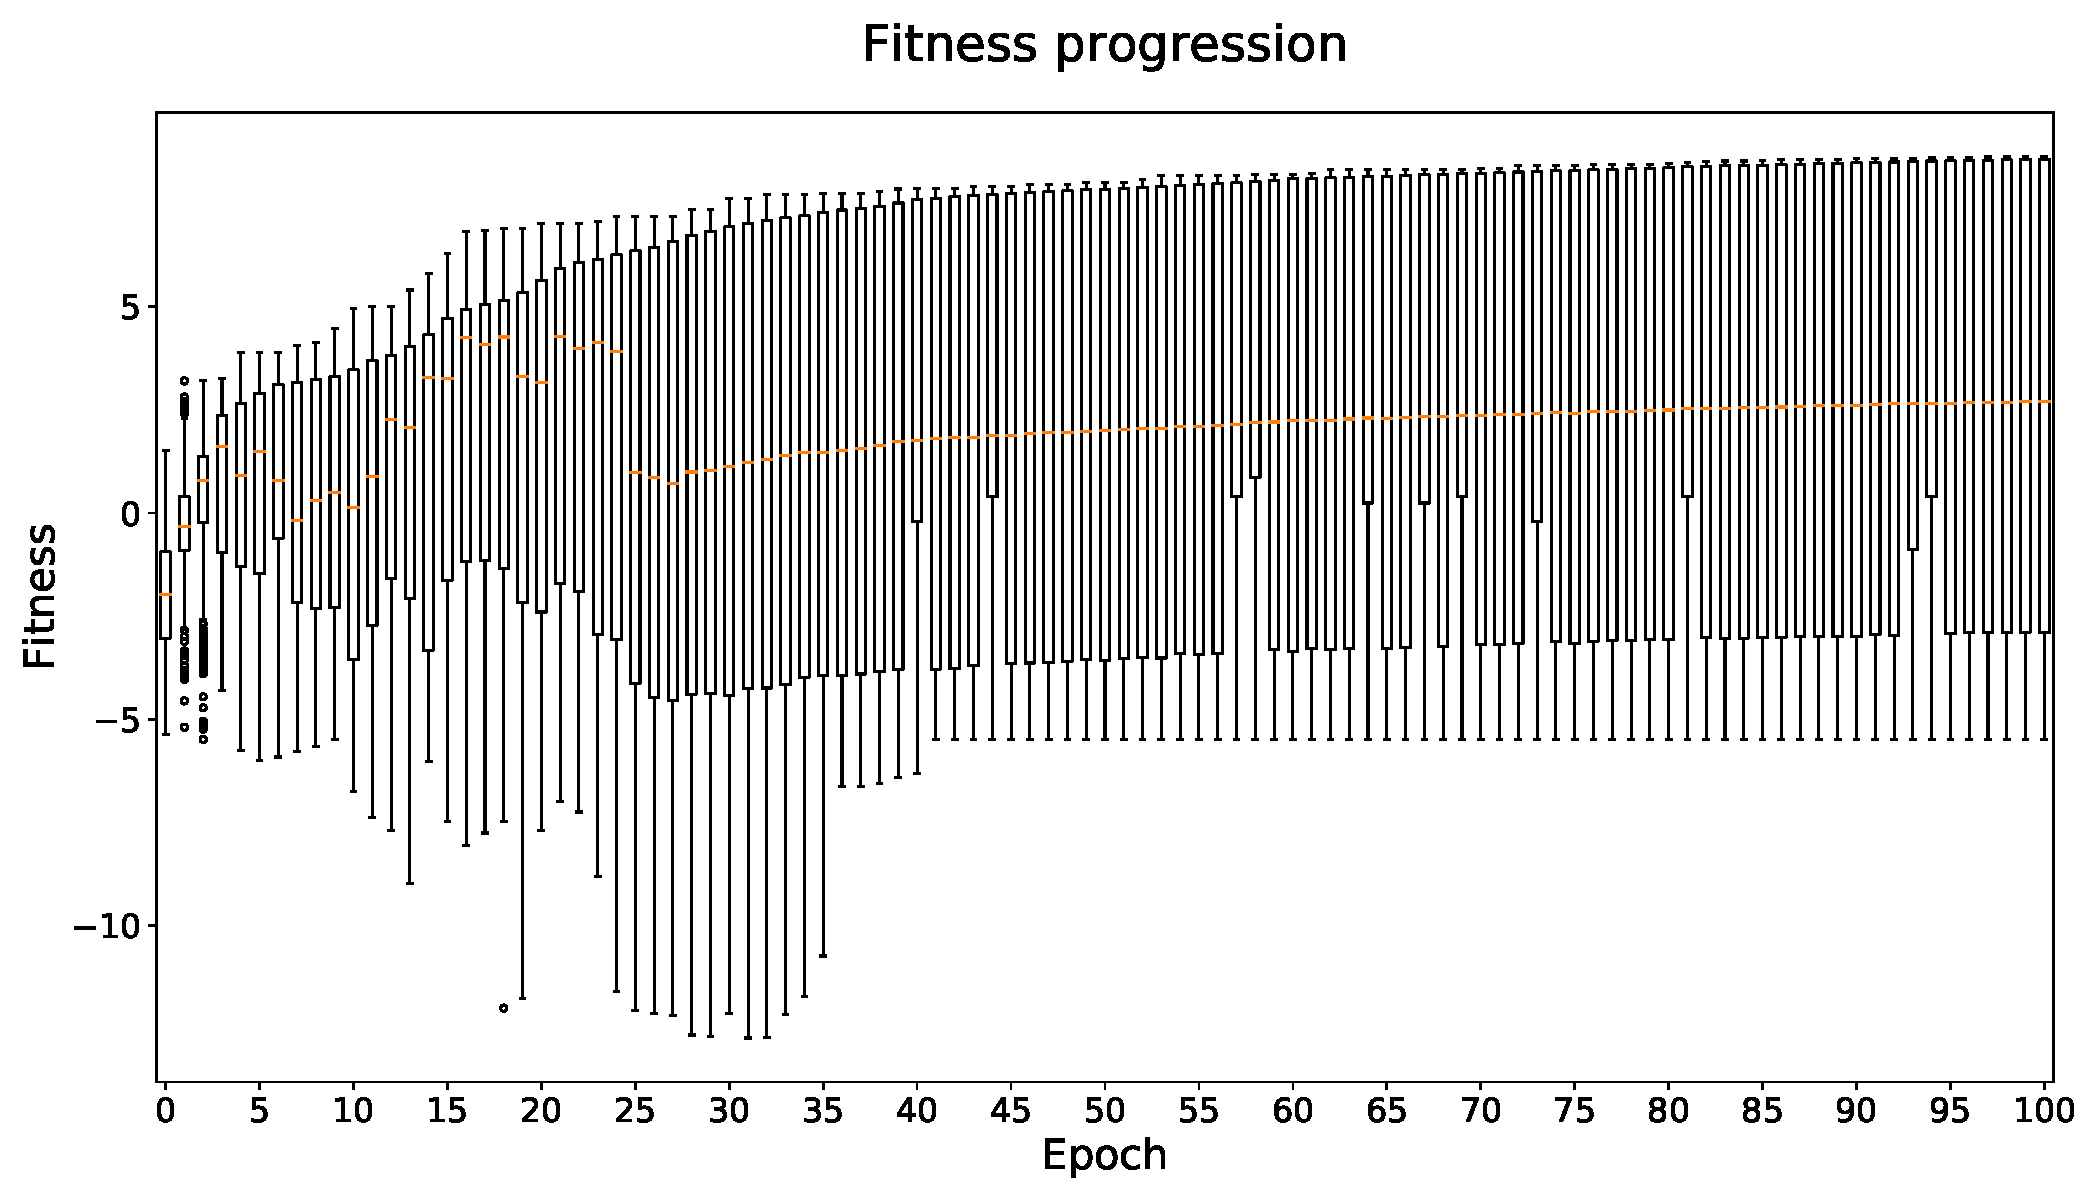
\includegraphics[width=.9\paperwidth]{img/circle/fitness.pdf}
    }
}

\frame{%
    \centering
    \begin{figure}
        \animategraphics[%
            loop,controls,width=\textwidth%
        ]{1}{img/circle/epoch_}{0}{100}
    \end{figure}
}



\frame{%
    Given:
    \begin{itemize}
        \item a large column, \(X\);
        \item some sampling proportion, \(p \in [0, 1]\);
        \item a number of samples to take, \(k\)
    \end{itemize}

    \alert{Minimise}
    \begin{itemize}
        \item[] The maximum sampled mean of \(X\)
    \end{itemize}
}

\frame{%
    \makebox[\linewidth]{%
        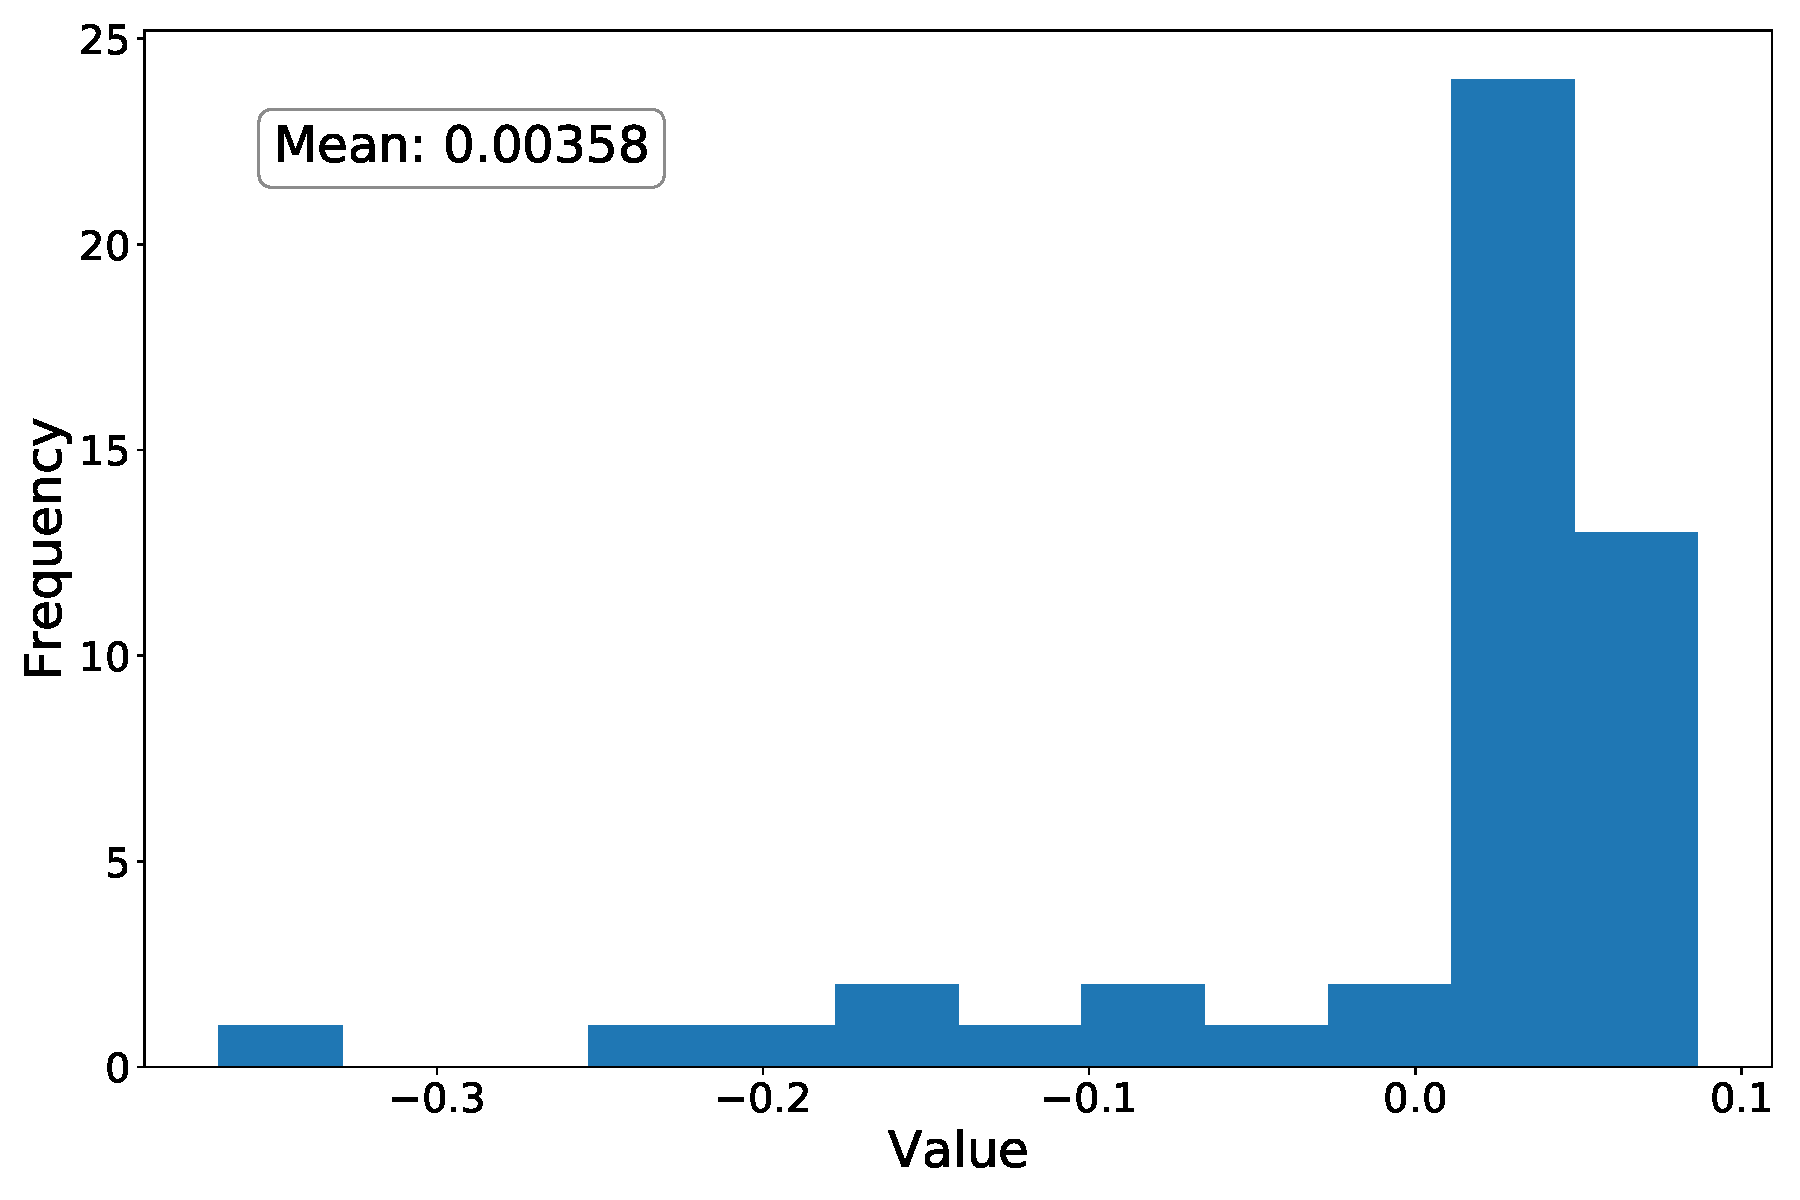
\includegraphics[width=.9\paperwidth]{img/sample_mean.pdf}
    }
}

\frame{%
    \centering
    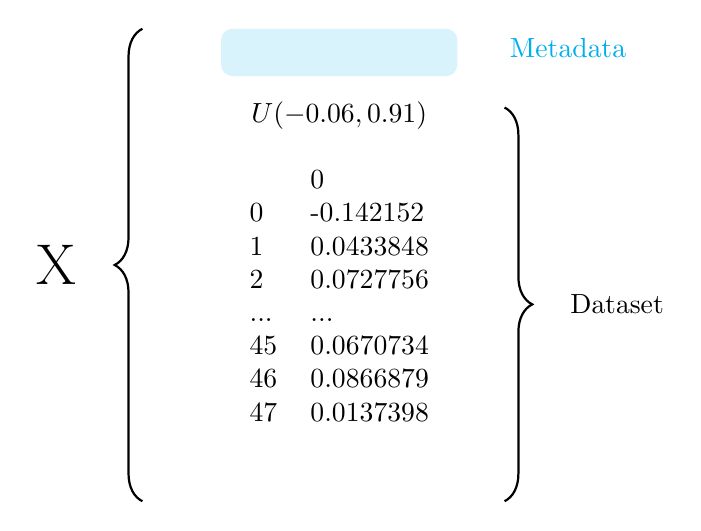
\begin{tikzpicture}

        \fill[cyan!15, rounded corners] (-1.5, 2.4) rectangle (1.5, 3)
            node[right=40pt, below] {\color{cyan} Metadata};
        \node at (0, 0) {%
            \begin{tabular}{c}
                \(U(-0.06, 0.91)\)\\
                {}\\
                \begin{tabular}{ll}
\toprule
{} &          0 \\
\midrule
0   &  -0.142152 \\
1   &  0.0433848 \\
2   &  0.0727756 \\
... &        ... \\
45  &  0.0670734 \\
46  &  0.0866879 \\
47  &  0.0137398 \\
\bottomrule
\end{tabular}

            \end{tabular}
        };

        \draw[decorate, decoration={brace, amplitude=10pt}, thick]%
            (-2.5, -3) -- (-2.5, 3) node[midway, left=20pt] {\huge X};
        \draw[decorate, decoration={brace, amplitude=10pt}, thick]%
            (2.1, 2) -- (2.1, -3) node[midway, right=20pt] {Dataset};
    \end{tikzpicture}
}

\frame{%
    Given a set of \(k\) \alert{dissimilarity} measures:
    \[
        f_1, \ldots, f_k: \mathbb{R}^n \times \mathbb{R}^n \to \mathbb{R}
    \]

    \alert{Minimise} their sum
}

\frame{%
    \makebox[\linewidth]{%
        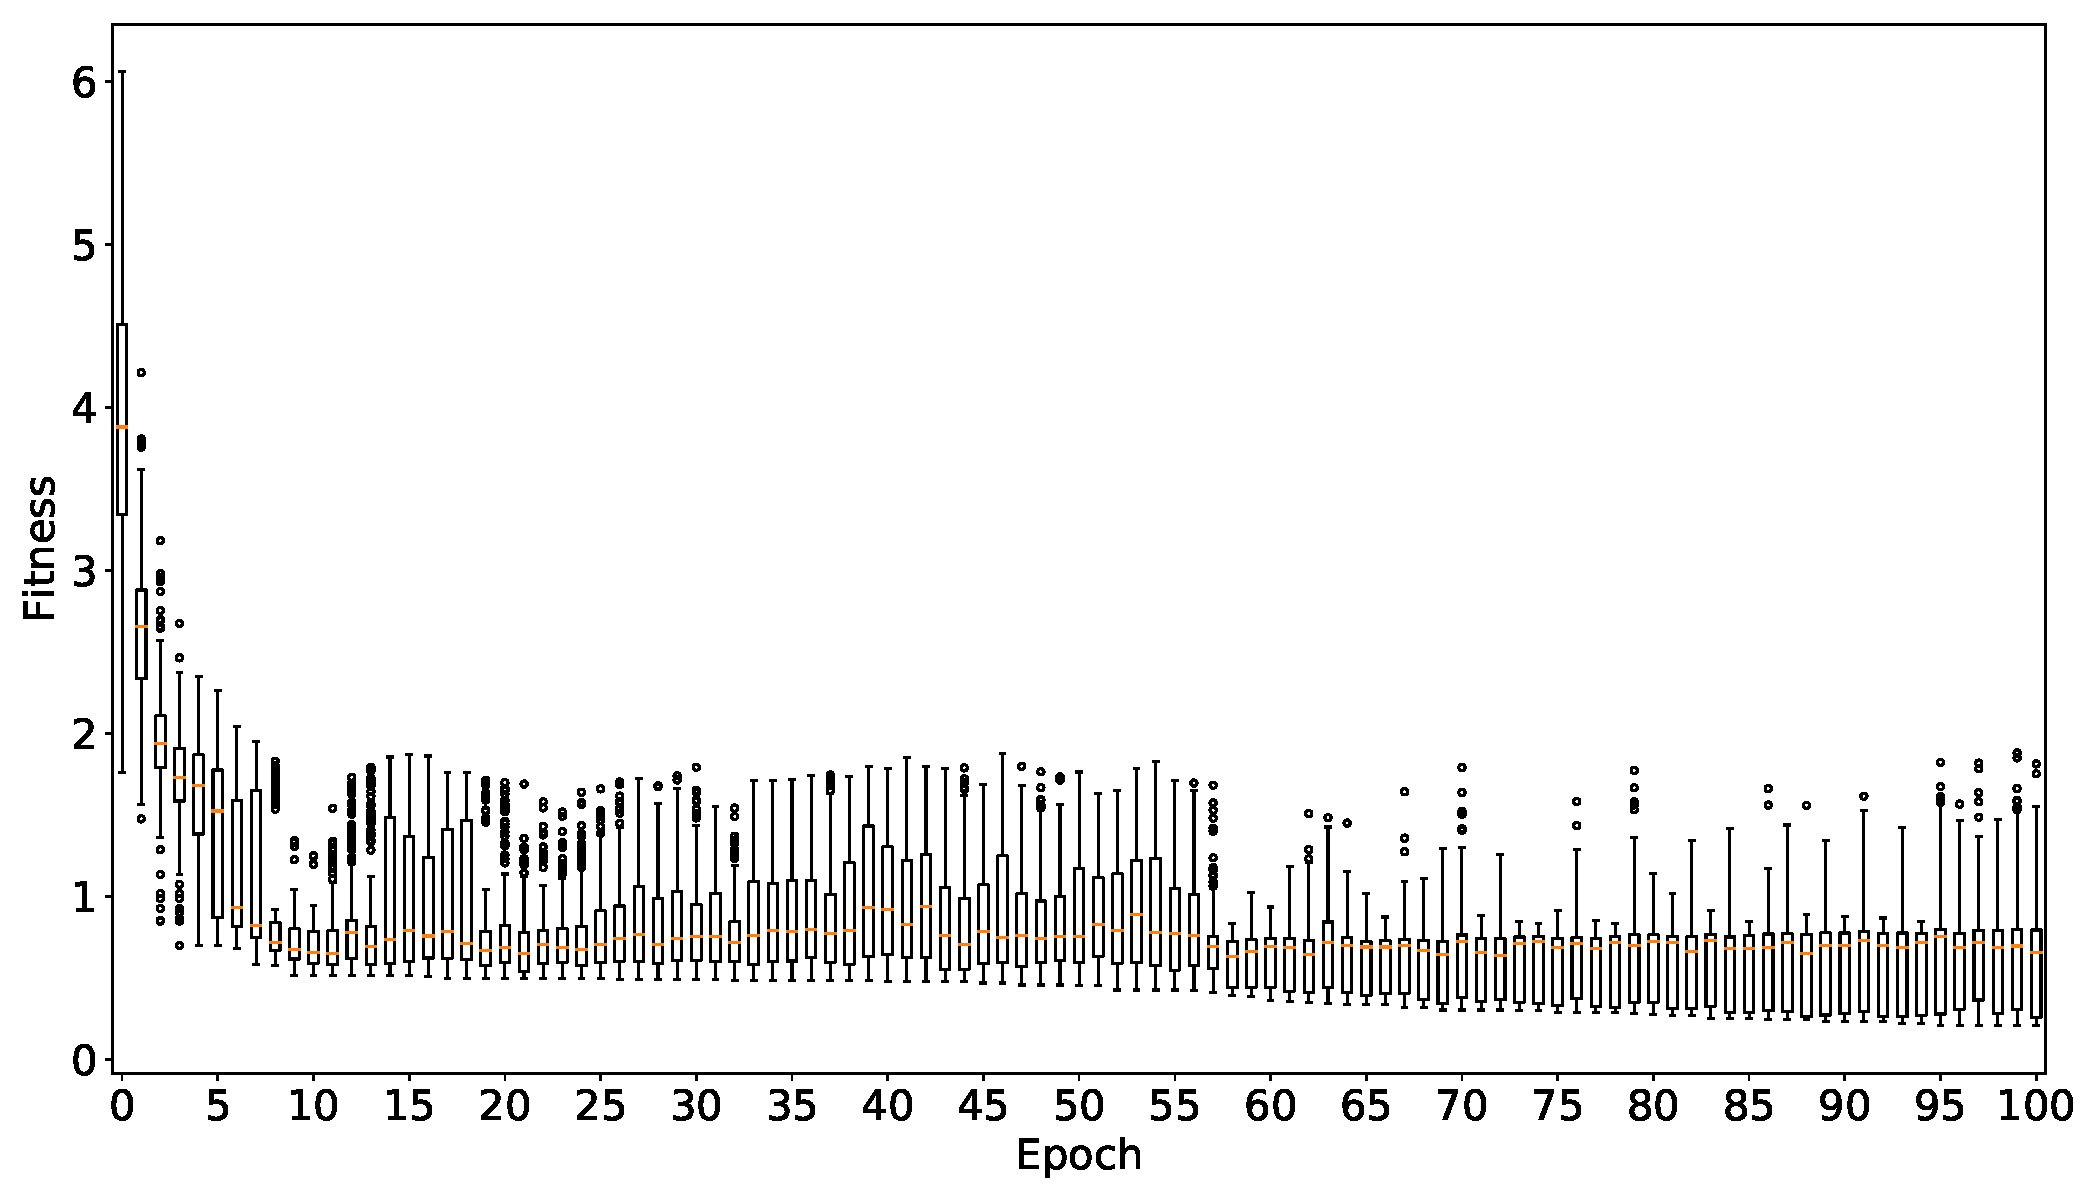
\includegraphics[width=.9\paperwidth]{img/anscombe/fitness.pdf}
    }
}

\frame{%
    \centering{%
        \(X\) Mean: 5 \hfill%
        \(Y\) Mean: 7 \hfill%
        \(X\) Std.: 4.7 \hfill%
        \(Y\) Std.: 4.1 \hfill%
        Corr.: 0.8
    }\vfill

    \begin{minipage}{\linewidth}
        \hspace*{-30mm}
        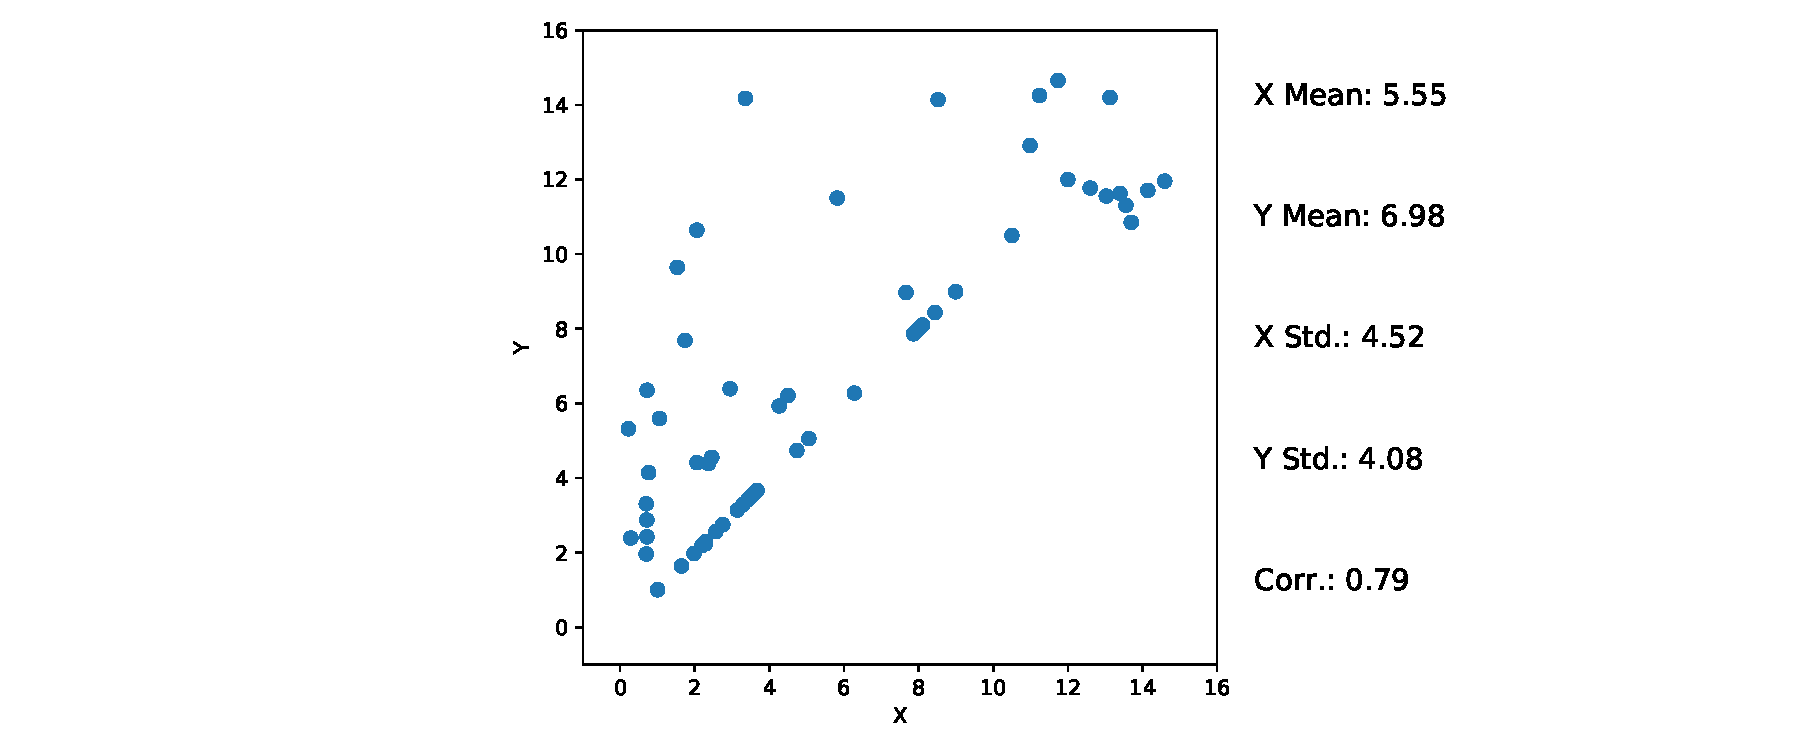
\includegraphics[height=.4\paperheight]{img/anscombe/best_0.pdf}%
        \hspace*{-30mm}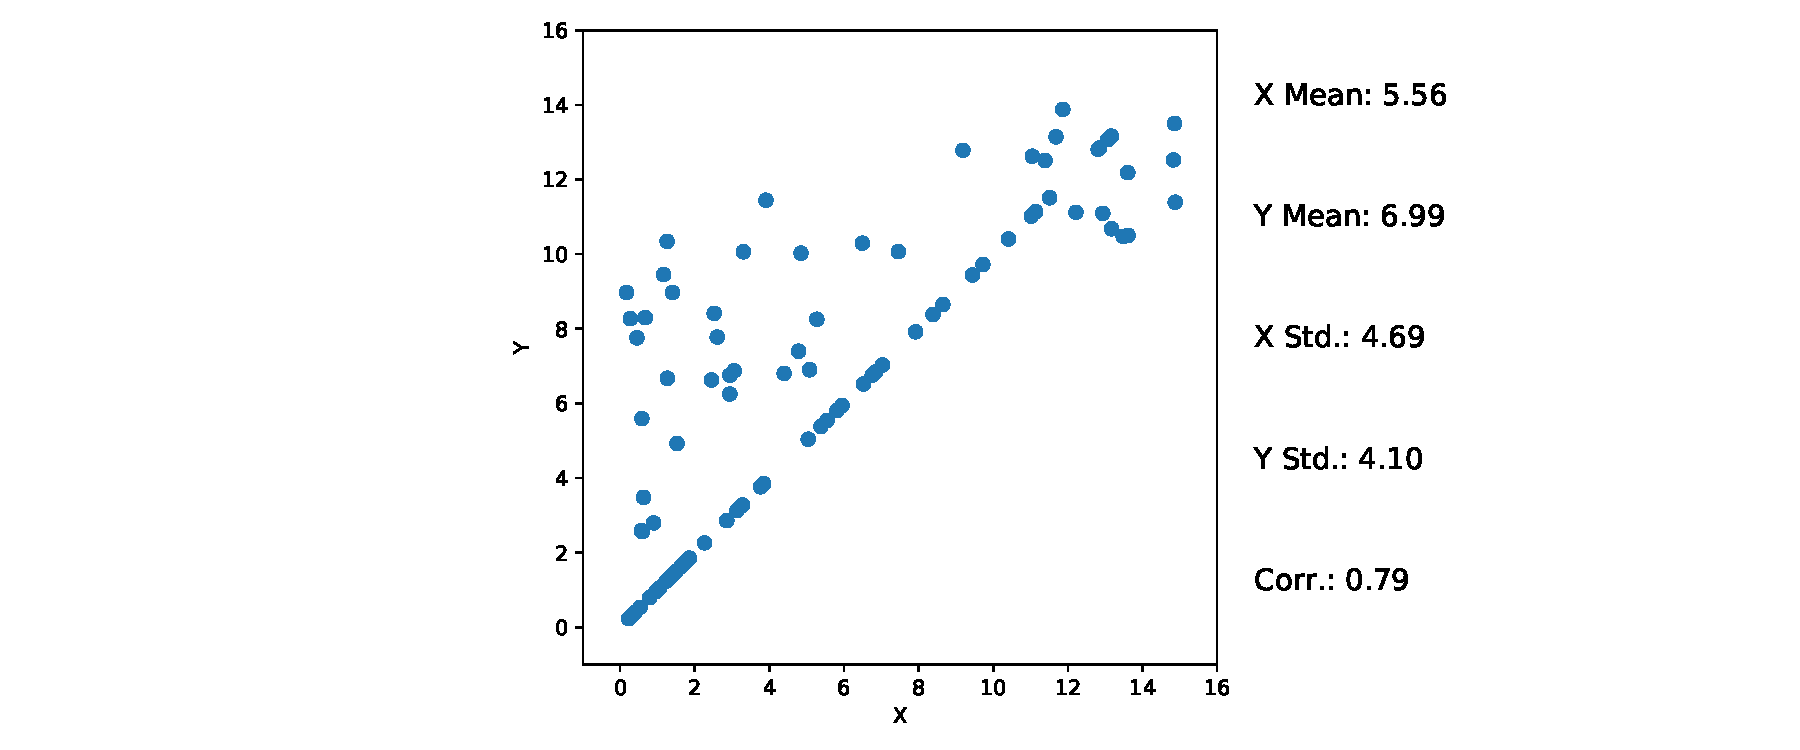
\includegraphics[height=.4\paperheight]{img/anscombe/best_1.pdf}
    \end{minipage}
    \begin{minipage}{\linewidth}
        \hspace*{-30mm}
        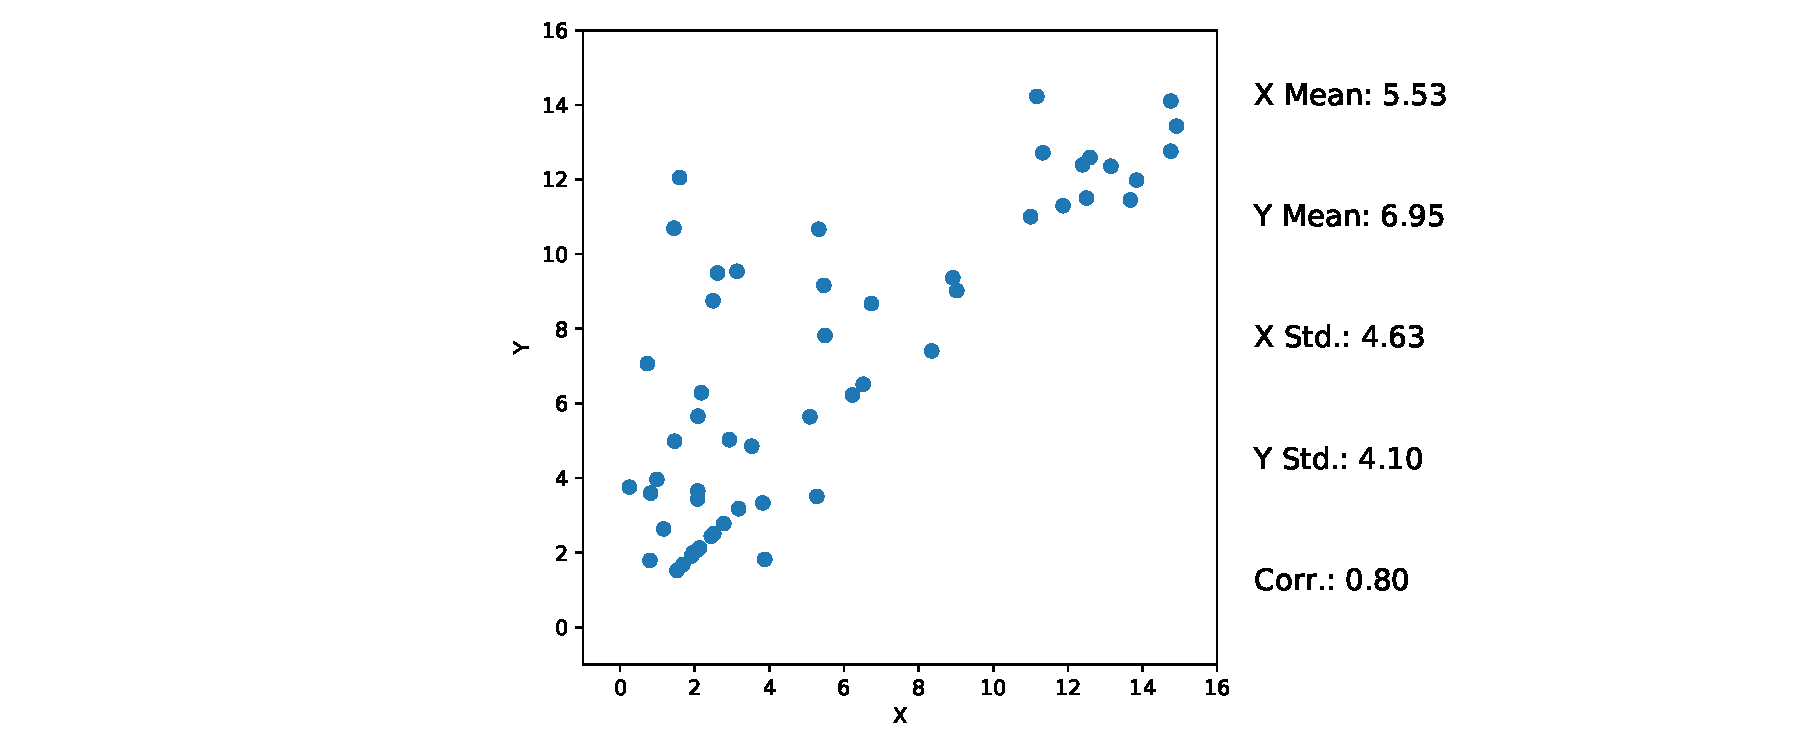
\includegraphics[height=.4\paperheight]{img/anscombe/best_2.pdf}%
        \hspace*{-30mm}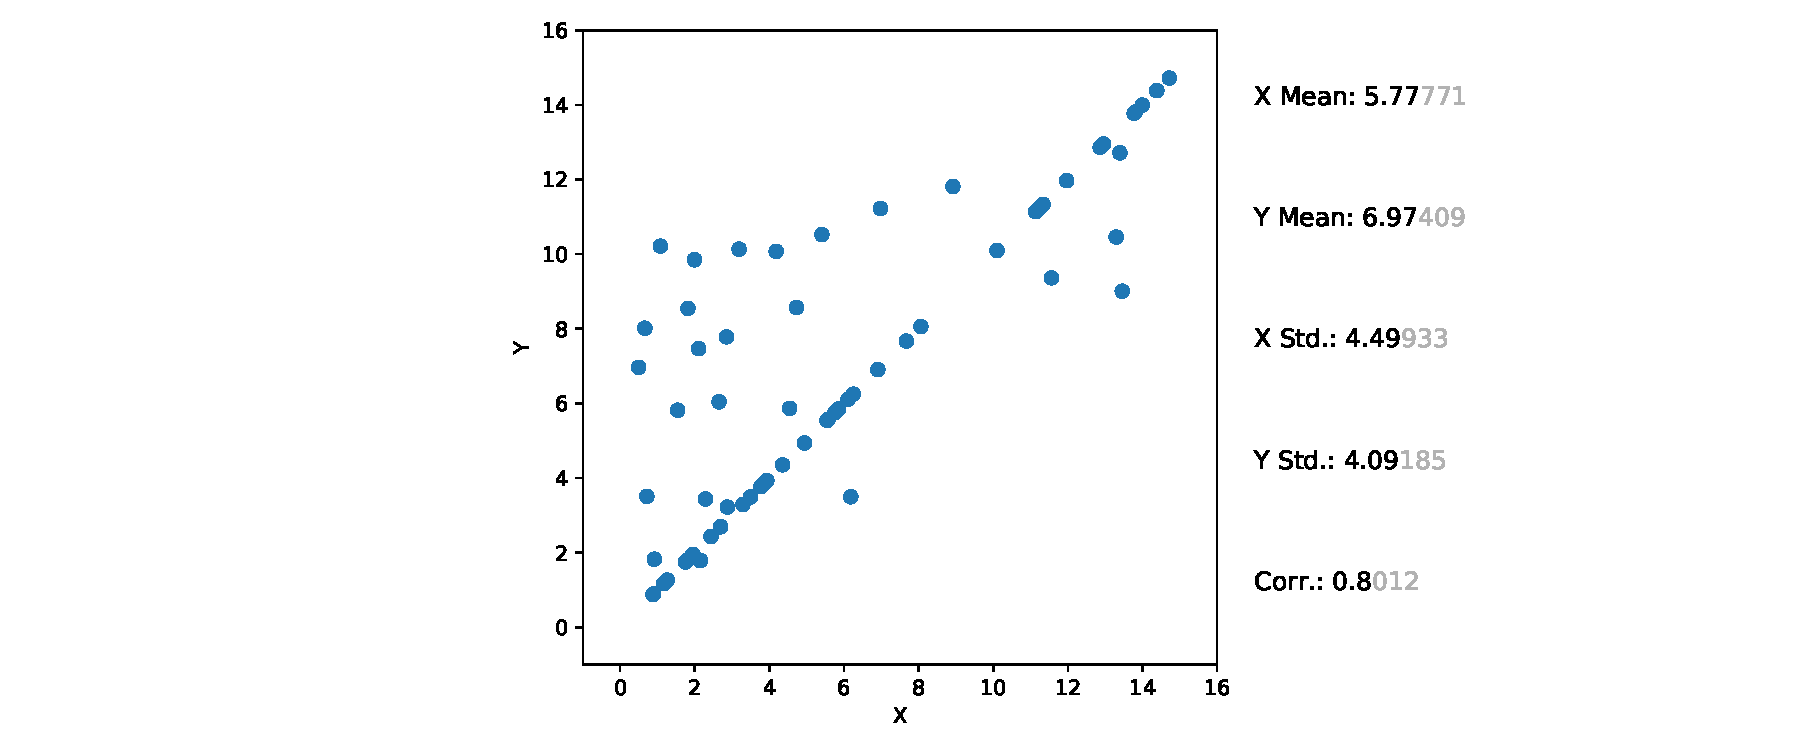
\includegraphics[height=.4\paperheight]{img/anscombe/best_3.pdf}
    \end{minipage}
}



\hammerpage%
